\section{Layers vs Tiers}
Typically an information system is constituted by three layers : presentation, application logic and resource management layer. The \textbf{presentation layer} is devoted to present the system's user interface to clients. The \textbf{application logic} determines what the system actually does. It takes care of enforcing business processes. The application logic can take many forms : programs, constraints, etc. The \textbf{resource manager} deals with the organization (storage, indexing and retrieval) of the data necessary to support the application logic. This is typically a database but it can also be a text retrieval system or any other data management system providing querying capabilities and persistence. A client is any user or program that wants to perform an operation over the information system. Clients are independent of each other : one could have several presentation layers depending on what each client wants to do. One can take advantage of the computing power at the client machine to have more sophisticated presentation layers. This also saves computer resources at the server machine. It introduces the concept of API, an interface to invoke the system from the outside. It also allow designers to think about federating the systems into a single system. The resource manager only sees one client : the application logic. This improve a lot the performance since there aren't client connections/session to maintain. A \textbf{tier} is a physical level. How can we divide logical layers over physical objects ? The first architecture developed is the so called \textbf{1-tier architecture}, in which all layers are running on the same machine (i.e. a mainframe). The second approach is called \textbf{2-tier architecture}, in which we can have one machine (server) that contains the application logic and resource management and another one (client) that contains the presentation layer. This approach is also called client-server architecture. The evolution of this concept is to introduce micro services, and using a \textbf{3-tier architecture}, in which the presentation layer runs on the client machine, the application logic layer on a middle machine and the resource management layer on a dedicated machine. The problem is that now, we have more connections respect to the previous architectures. In fact, the middle's developers needs to write the code for  receiving requests from the client and from the server. So, the people realize that needed something more, a specific technologies called \textbf{middleware}, that could make the development of the code as much simple as if the code is still running in the mainframe (on the same machine). Once you know how to split the software in three layers, you can split each of them in more layers on its own machine, in order to make load balance. The result of this idea is called \textbf{N-tier architecture}.
\subsection{Middleware}
A middleware can serves the requests in two ways :
\begin{itemize}
    \item \textbf{Synchronous} : traditionally, distributed applications use blocking calls, in which the client sends a request to a service and waits for a response of the service to come back before continuing doing its work. This type of interaction require both parties to be online : the client make the request, the receiver gets the request, processes it and sends a response to the caller, the client receives the response. Due it synchronizes client and server, this approach has several disadvantages :
          \begin{itemize}
              \item \textbf{connection overhead} : synchronous invocations require to maintain a session between the caller and the receiver. Maintaining a session is expensive and consumes CPU resources. There is also a limit on the number of session that can be active at the same time. For this reason, client/server systems often use connection pooling (pooling of connections, with a thread associate at each of them and allocate one of them when needed) to optimize resource utilization. Synchronous interaction requires a context for each call and a context management system for all incoming calls. The context needs to be passed around with each call as it identifies the session, the client and the nature of the interaction.
              \item \textbf{higher probability of failures} : if the client or the server for some reason fail, the context is lost and resynchronization is difficult. Finding out when the failure took place may not be easy.
          \end{itemize}
          To the previous problems there are two solutions :
          \begin{itemize}
              \item \textbf{Enhanced support} : we can use transactional interaction to enforce exactly once execution semantics and enable more complex interactions with some executions guarantees. Another approach is service replication and load balancing, in order to prevent the service from becoming unavailable when there is a failure.
              \item \textbf{Asynchronous interaction} : see below.
          \end{itemize}
    \item \textbf{Asynchronous} : using asynchronous interaction, the caller sends a message that gets stored somewhere until the receiver reads it and sends a response. The response is sent in a similar manner as before. This type of interaction can take place in two forms :
          \begin{itemize}
              \item \textbf{non-blocking invocation} : a service invocation but the call returns immediately without waiting for a response, similar to batch jobs.
              \item \textbf{persistent queue} : the call and the response are actually persistently stored until they are accessed by the client and the server.
          \end{itemize}
\end{itemize}
A middleware can be implemented with two approaches :
\begin{itemize}
    \item \textbf{Programming abstraction} : it's an approach intended to hide low level details of hardware, network and distribution. Middleware is primarily a set of programming abstractions developed to facilitate the development of complex distributed systems; to understands a middleware platform one needs to understand its programming model. From this latter can be determined its limitations, general performance and applicability of a given type of middleware. Furthermore, this model also determines how the platform will evolve.
    \item \textbf{Infrastructure} : as the programming abstraction reach higher and higher levels, also the infrastructure that implements the abstractions must grow accordingly. Additional functionality is always implemented through additional software layer. The additional software layers increase the size and the complexity of the infrastructure necessary to use the new abstractions. The infrastructure is also intended to support additional functionality that makes development, maintenance and monitoring easier and less costly. It takes care of all non-functional properties typically ignored by programming models and languages such as performance, maintenance, resource management, etc.
\end{itemize}
Typically a middleware is based on RPC, in which the client invoke a local procedure talking with its stub (client stub), which is able to communicate with the remote object via a communication module. A request is created putting the client parameters, serialized (marshal operation) and send to the server stub. The server dispatcher deliver the serialized request to its stub, which deserialize (unmarshal operation) it, extract the parameters and finally call the server procedure. When there are more entities interacting with each other, RPC treats the calls as independent of each other. The main drawback of RPC is that recovering from partial system failures may be very complex. So, a programmer instead to implement the whole infrastructure for a distributed application can use an RPC system, which hides distribution behind procedure calls, provides an interface definition language (IDL) to describe the services, generates all the additional code necessary to make a procedure call remote and to deal with all the communication aspects and provides a binder in case it has a distributed name and directory service system. The solution to this limitation is to make RPC calls transactional, i.e. instead of providing plain RPC, the system should provide TRPC. It's based on the same concepts of RPC but, use additional language constructs and runtime support to bundle several RPC calls into an atomic unit.
\subsubsection{Message Oriented Middleware}
MOM is software or hardware infrastructure supporting sending and receiving messages between distributed systems, with the following structure :

\begin{center}
    %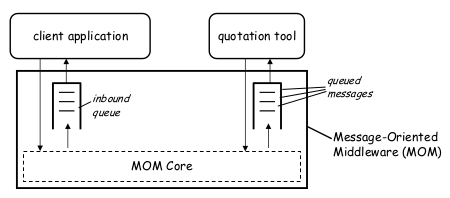
\includegraphics[scale=0.55]{images/MOM_schema.png}
\end{center}
The participants of the communication are divided into two groups :
\begin{itemize}
    \item \textbf{Publisher} : the entity that send messages
    \item \textbf{Subscriber} : the entity that express interest in certain categories of messages.
\end{itemize}
The main disadvantage of this approach is that require an extra component in the architecture called \textbf{event service} that receives messages from publisher and cross-check them with the interests of subscribers. As with any system, an introduction of another component can lead to performance and reliability reduction, and can make the whole system more difficult and expensive to maintain. The information can be processed in two ways :
\begin{itemize}
    \item \textbf{Topic-based} : the publisher is responsible for defining the topics to which subscribers can subscribe.
    \item \textbf{Content-based} : filters can be used for a more accurate selection of information to be received.
\end{itemize}
The publisher can specify which topics are available for a subscription (topic-based) and subscribers can specify particular attribute in order to filtering the messages of interest.
The notification can be made in two ways :
\begin{itemize}
    \item \textbf{push} : the subscribers are invoked in callback, using a reference communicated at the time of subscription.
    \item \textbf{pull} : the subscribers poll the event service when they need messages.
\end{itemize}
\hl{To-Do : add the pseudocode !}
